\hebrewsection{Detection and Demodulation}

\subsection{The Optimal Receiver}
In an AWGN (Additive White Gaussian Noise) channel, the optimal receiver maximizes the likelihood of the correct symbol.

\subsubsection{The Matched Filter}
The matched filter $h(t) = s(T-t)$ maximizes the SNR at the sampling instant. This is equivalent to a correlator receiver.
\begin{equation}
    h(t) = s^*(T-t)
\end{equation}
The output of the matched filter at $t=T$ is exactly the inner product $\langle r, s \rangle$.

\begin{pythonbox}{BER Simulation for BPSK}
\begin{verbatim}
import numpy as np

def simulate_ber(ebno_db, n_bits=1000000):
    ebno = 10**(ebno_db / 10)
    sigma = np.sqrt(1 / (2 * ebno))
    
    bits = np.random.randint(0, 2, n_bits)
    tx = 2 * bits - 1  # BPSK: 0 -> -1, 1 -> 1
    
    noise = sigma * np.random.randn(n_bits)
    rx = tx + noise
    
    # Decisions
    decisions = (rx > 0).astype(int)
    errors = np.sum(decisions != bits)
    return errors / n_bits
\end{verbatim}
\end{pythonbox}

\subsection{Probability of Error Analysis}
The Bit Error Rate (BER) depends on the distance between constellation points and the noise power.

\subsubsection{BER for BPSK}
\begin{equation}
    P_b = Q\left(\sqrt{\frac{2E_b}{N_0}}\right)
\end{equation}
The Q-function $Q(x)$ is the tail probability of the standard normal distribution.

\subsection{Coherent vs. Non-Coherent Demodulation}
Coherent demodulation requires carrier phase knowledge, while non-coherent (e.g., envelope detection for FSK) does not. Coherent systems perform better but are more complex.

\subsection{BER Performance Graphs}
The following graph shows the theoretical BER for different modulation schemes. Note the SNR penalty for higher-order modulation.

\begin{center}
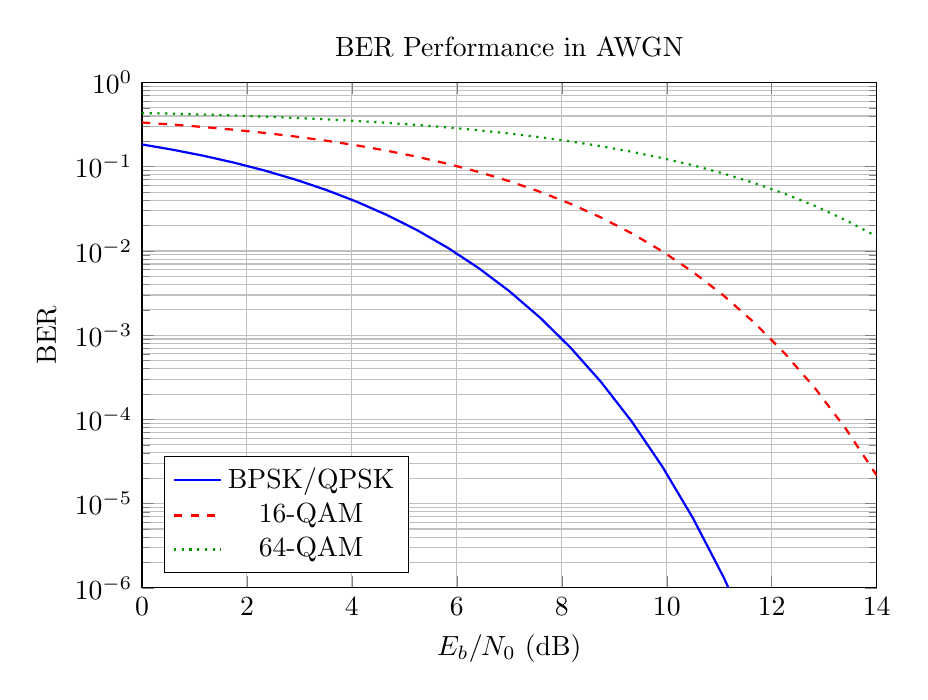
\begin{tikzpicture}
\begin{axis}[
    title={BER Performance in AWGN},
    xlabel={$E_b/N_0$ (dB)},
    ylabel={BER},
    ymode=log,
    grid=both,
    xmin=0, xmax=14,
    ymin=1e-6, ymax=1,
    width=0.9\textwidth,
    height=8cm,
    legend pos=south west
]
% Approximation for Q-function: Q(x) ~ 0.5 * exp(-x^2 / 2)
\addplot[blue, thick, domain=0:14] {0.5 * exp(-10^(x/10))};
\addlegendentry{BPSK/QPSK}
\addplot[red, thick, dashed, domain=0:14] {0.5 * exp(-0.4 * 10^(x/10))};
\addlegendentry{16-QAM}
\addplot[green!60!black, thick, dotted, domain=0:14] {0.5 * exp(-0.14 * 10^(x/10))};
\addlegendentry{64-QAM}
\end{axis}
\end{tikzpicture}
\end{center}

\subsection{Decision Boundaries}
For an $M$-ary constellation, the receiver divides the I-Q plane into $M$ decision regions. Any received point within a region is mapped to the corresponding symbol.

\subsection{Maximum Likelihood Sequence Estimation (MLSE)}
For channels with memory or ISI, symbol-by-symbol detection is sub-optimal. The \textbf{Viterbi Algorithm} provides the MLSE by efficiently searching the trellis of possible transmitted sequences.

\subsection{Gray Coding}
Gray coding ensures that adjacent constellation points differ by only one bit. This minimizes the bit error rate for a given symbol error rate.
